\documentclass[border=8pt]{standalone}
\usepackage{amsmath}
\usepackage{tikz}
\usetikzlibrary{arrows.meta,positioning,calc,fit}
\begin{document}
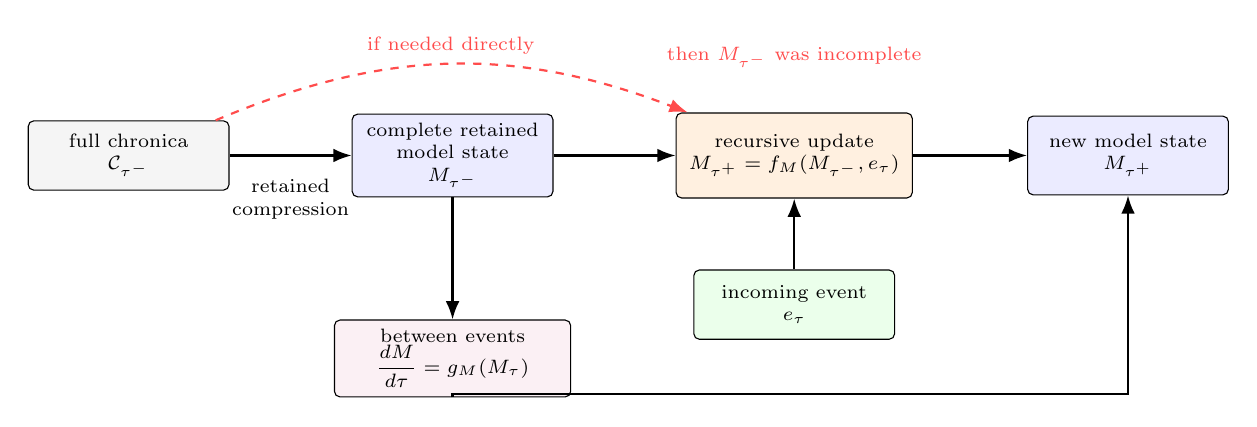
\begin{tikzpicture}[
  box/.style={draw, rounded corners=2pt, align=center, minimum width=2.55cm, minimum height=0.88cm, font=\scriptsize},
  state/.style={draw, rounded corners=2pt, align=center, minimum width=2.55cm, minimum height=1.0cm, font=\scriptsize, fill=blue!8},
  update/.style={draw, rounded corners=2pt, align=center, minimum width=3.0cm, minimum height=1.08cm, font=\scriptsize, fill=orange!12},
  note/.style={align=center, font=\scriptsize},
  arr/.style={-Latex, thick},
  dasharr/.style={-Latex, thick, dashed}
]

\node[box, fill=gray!8] (chronica) {full chronica\\$\mathcal C_{\tau^-}$};
\node[state, right=1.55cm of chronica] (model) {complete retained\\model state\\$M_{\tau^-}$};
\node[update, right=1.55cm of model] (upd) {recursive update\\$M_{\tau^+}=f_M(M_{\tau^-},e_\tau)$};
\node[box, fill=green!8, below=0.9cm of upd] (event) {incoming event\\$e_\tau$};
\node[state, right=1.45cm of upd] (next) {new model state\\$M_{\tau^+}$};

\draw[arr] (chronica) -- (model);
\node[note, below=0.18cm of $(chronica)!0.5!(model)$] {retained\\compression};
\draw[arr] (model) -- (upd);
\draw[arr] (event) -- (upd);
\draw[arr] (upd) -- (next);

\draw[dasharr, red!70] (chronica) to[bend left=22] node[above, font=\scriptsize, text=red!70] {if needed directly} (upd);
\node[note, text=red!70, above=0.45cm of upd] {then $M_{\tau^-}$ was incomplete};

\node[box, fill=purple!6, below=1.55cm of model, minimum width=3.0cm] (between) {between events\\$\dfrac{dM}{d\tau}=g_M(M_\tau)$};
\draw[arr] (model) -- (between);
\draw[arr] (between) -- ++(0,-0.45) -| (next);

\end{tikzpicture}
\end{document}
